% This is LLNCS.DEM the demonstration file of
% the LaTeX macro package from Springer-Verlag
% for Lecture Notes in Computer Science,
% version 2.4 for LaTeX2e as of 16. April 2010
%
\documentclass{llncs}
%
\usepackage{makeidx}  % allows for indexgeneration
\usepackage{llncsdoc}
\usepackage{algorithmic}
\usepackage{amssymb}
\usepackage{graphicx}
\usepackage{wrapfig}
\usepackage{cite}
\usepackage{amsmath}
\usepackage[usenames,dvipsnames]{xcolor}
\usepackage[parfill]{parskip} 
\usepackage{float}
\usepackage{caption}
%\restylefloat{table}

\newcommand{\Mod}[1]{\ (\text{mod}\ #1)}
\newcommand{\todo}[1]{{\color{red}{TODO #1}}}
\renewcommand\refname{Referin\c{t}e}
\setcounter{secnumdepth}{4}
\def\examplename{Exemplul}
\def\contentsname{Cuprins}
\captionsetup[table]{name=Tabel}

%
\begin{document}
\pagestyle{empty}
%
%
\title{TODO}
%
\titlerunning{Research report for UROP course}  % abbreviated title (for running head)
%                                     also used for the TOC unless
%                                     \toctitle is used
%
\subtitle{- Undergraduate Research Opportunities - }
\author{Drago\c{s} Alin Rotaru.\\{\small \textbf{Mentor}: Ruxandra F. Olimid}}
\authorrunning{D.A.Rotaru} % abbreviated author list (for running head)
%
%%%% list of authors for the TOC (use if author list has to be modified)
%\tocauthor{}

\institute{Universitatea din Bucure\c{s}ti \\ ROMANIA\\
\email{r.dragos0@gmail.com
}
}


\maketitle              % typeset the title of the contribution

\begin{abstract}
TODO - abstract
%\keywords{securitate, scheme de partajare}
\end{abstract}

\tableofcontents
\newpage
%----------------------------------------------------------------
%----------------------------------------------------------------
%----------------------------------------------------------------
%----------------------------------------------------------------
%----------------------------------------------------------------

\section{Introducere}
\label{sec:intro}

\subsection{Istoric}
Termenul de criptografie este definit in dic\c{t}ionarul Oxford ca fiind \textit{arta de a scrie \c{s}i a rezolva coduri}.
Criptografia moderna s-a desprins de cea clasica \^{i}n jurul anilor '80, motiv\^{a}nd implementarea rigurozit\u{a}\c{t}ii matematice pentru definirea construc\c{t}iilor criptografice. Asta pentru ca \^{i}n anii anteriori, experien\c{t}a a dovedit nesiguran\c{t}a metodelor de criptare, criptanaliza lor fiind uneori trivial\u{a} (cifrul lui Cezar, Vigenere \cite{Caesar:2015}, \cite{Vigenere:2015}) sau uneori atins\u{a} cu ceva mai mult efort precum Enigma \c{s}i alte metode din cel de-al doilea r\u{a}zboi mondial \cite{Enigma:2015}.

Criptografia modern\u{a} se gase\c{s}te pretutindeni \^{i}n via\c{t}a de zi cu zi de la ATM-uri, cartele telefonice la semn\u{a}turi digitale, protocoale de autentificare, licita\c{t}ii electronice sau bani digitali, lu\^{a}nd amploare o dat\u{a} cu apari\c{t}ia sistemelor cu cheie public\u{a}. O defini\c{t}ie potrivit\u{a} este \textit{studiul \c{s}tiin\c{t}ific al tehnicililor pentru a securiza informa\c{t}ia digital\u{a}, tranzac\c{t}iile \c{s}i calculul distribuit.} \cite{Katz:2007}.

\subsection{Motiva\c{t}ie}

O schem\u{a} de partajare este o metod\u{a} de a distribui un secret unor participan\c{t}i, oferind fiec\u{a}rui participant o component\u{a} (share) a.\^{i}. doar o submul\c{t}ime de participan\c{t}i pot recupera secretul. Schemele de partajare sunt protocoale criptografice versatile \c{s}i sunt folosite in multe aplica\c{t}ii precum: protejarea / recuperarea cheilor criptografice, vot electronic, certificate distribuite unor autorit\u{a}\c{t}i, licita\c{t}ii on-line sau sisteme de stocare de lung\u{a} durat\u{a} \cite{Martin:2008}.


\subsection{Structur\u{a}}
\begin{itemize}
	\item Sec\c{t}iunea {\ref{sec:intro}} descrie pe scurt obiectul de studiu.
	\item Sec\c{t}iunea {\ref{sec:splitting_schemes}} ofer\u{a} o scurt\u{a} introducere \^{i}n domeniul schemelor de partajare \c{s}i descrie \^{i}n detaliu metodele ce vor fi folosite \^{i}n sec\c{t}iunile urm\u{a}toare.
	\item Sec\c{t}iunea {\ref{sec:long_term_systems_intro}} con\c{t}ine no\c{t}iuni introductive despre sistemele de stocare de lung\u{a} durat\u{a}.
	\item Sec\c{t}iunea {\ref{sec:long_term_systems_full}} descrie c\^{a}teva sisteme considerate relevante pentru \^{i}ntelegerea contribu\c{t}iilor p\^{a}n\u{a} \^{i}n prezent.
	\item Sec\c{t}iunea {\ref{sec:desc_alouneh}} introduce sistemul criptanalizat.
	\item Sec\c{t}iunea {\ref{sec:obtained_results}} con\c{t}ine contribu\c{t}iile de cercetare pun\^{a}nd \^{i}n eviden\c{t}\u{a} determinismul prezent al sistemului introdus \^{i}n Sec\c{t}iunea {\ref{sec:desc_alouneh}}.
\end{itemize}

%----------------------------------------------------------------
%----------------------------------------------------------------
%----------------------------------------------------------------
%----------------------------------------------------------------
\section{Scheme de partajare}
\label{sec:splitting_schemes}

%TODO: find translation for multi party computation

O schem\u{a} de partajare const\u{a} \^{i}n distribuirea unei informa\c{t}ii secrete $\mathcal{S}$ la mai mul\c{t}i participan\c{t}i $\mathcal{P} = \{P_1, \dots, P_n\}$ astfel \^{i}nc\^{a}t oricare mul\c{t}ime de participan\c{t}i predefinit\u{a}  ca f\u{a}c\^{a}nd parte dintr-o structur\u{a} de acces pe care o vom denumi $\mathcal{A}$ s\u{a} poat\u{a} reconstitui secretul $\mathcal{S}$.
Formal, o schem\u{a} de partajare este reprezentat\u{a} de o pereche de algoritmi \textbf{$(Gen, Rec)$}:
\begin{itemize}
	\item \textit{$Gen(S, m)$} este un algoritm care prime\c{s}te la intrare un secret \textit{S} \c{s}i un num\u{a}r \^{i}ntreg $m$ \c{s}i \^{i}ntoarce un set de componente ${s_1, s_2, \dots, s_m}$.
	\item \textit{$Rec({s_i}_1, {s_i}_2, \dots, {s_i}_q)$} este un algoritm care prime\c{s}te ca parametri de intrare o mul\c{t}ime de componente \c{s}i \^{i}ntoarce \textit{S} dac\u{a} mul\c{t}imea $\{{P_i}_1, {P_i}_2, \dots, {P_i}_q \} \in \mathcal{A}$.
\end{itemize} 
%todo: add some more text between itemizers
Majoritatea schemelor constau \^{i}n mai multe etape precum:
\begin{itemize}
	\item \textit{Ini\c{t}ializare}. Presupune ini\c{t}ializarea variabilelor de mediu necesare.
	\item \textit{Generare}. O entitate autorizat\u{a} (numit\u{a} dealer) $\mathcal{D}$ folose\c{s}te algoritmul \textit{Gen} pentru a genera componentele.
	\item \textit{Distribu\c{t}ie}. Componentele sunt trimise participan\c{t}ilor cu ajutorul unui mijloc de comunicare sigur, f\u{a}r\u{a} ca acestea sa fie vizibile unui atacator.
	\item \textit{Reconstruc\c{t}ie}. D\^{a}ndu-se o mul\c{t}ime de componente, se folose\c{s}te algoritmul \textit{Rec} pentru a recupera secretul
	$\mathcal{S}$.
\end{itemize}

Schemele de partajare se clasific\u{a} in func\c{t}ie de cantitatea de informa\c{t}ie secret\u{a} pe care o pot ob\c{t}ine persoanele care nu fac parte din $\mathcal{A}$ \cite{Martin:2008}:
\begin{itemize}
	\item \textit{Sisteme perfecte de partajare}: componentele nu ofer\u{a} nici o informatie teoretic\u{a} despre $\mathcal{S}$ indiferent de resursele computa\c{t}ionale.
	\item \textit{Sisteme statistic sigure}: o frac\c{t}iune de informa\c{t}ie este dezvaluit\u{a} despre $\mathcal{S}$ independent de puterea computional\u{a} a adversarului.
	\item \textit{Sisteme computa\c{t}ional-sigure de partajare}: se bazeaz\u{a} pe faptul ca reconstituirea lui $\mathcal{S}$ se reduce la o problema \textit{dificil\u{a}} (spre exemplu problema Diffie-Hellman \cite{boneh:1998decision} ) \^{i}n lipsa unor informa\c{t}ii oferite doar grupului de acces $\mathcal{A}$.
%cite somehow AA article \todo{nu toate problemele sunt demonstrate ca fiind NP complete, se crede ca sunt probleme dificile}. ups, forgot about that:)
\end{itemize} 

\^{I}n continuare vom prezenta cateva sisteme perfecte de partajare utilizate \^{i}n cadrul unor arhitecturi pentru stocarea fisierelor pe o durata indelungat\u{a}.

\subsection{Istoric}

Primele scheme de partajare au fost dezvoltate independent de Shamir \c{s}i Blakley in 1979 \cite{B:1979, S:1979}.

Denumite \c{s}i scheme majoritare $(k, n)$, acestea rezolvau cazul \^{i}n care oricare grup de participan\c{t}i cu un num\u{a}r mai mare sau egal dec\^{a}t $k$  (m\u{a}rimea pragului) poate reconstitui secretul $\mathcal{S}$ din componentele primite de la dealer. Dac\u{a} schema este perfect \textit{sigur\u{a}} atunci oricare grup cu un num\u{a}r de participan\c{t}i mai mic decat $k$ nu ob\c{t}ine vreo informa\c{t}ie despre $\mathcal{S}$.


Schemele majoritare (spre exemplu schema Shamir) sunt insuficiente pentru a permite partajarea pentru anumite structuri de acces. Consider\u{a}m cazul \^{i}n care vrem sa partajam un secret \^{i}ntre 4 participan\c{t}i: $P_1, P_2, P_3, P_4$ astfel \^{i}nc\^{a}t $\{P_1,P_2\}$ \c{s}i $\{P_3,P_4\}$ s\u{a} fie singurele mul\c{t}imi autorizate pentru reconstruc\c{t}ia secretului $S$ (i.e. $\mathcal{A} = \{ \{P_1,P_2\}, \{P_3,P_4\} \}$). \^{I}n mod evident, problema nu poate fi rezolvat\u{a} cu o structur\u{a} de acces de tip prag: anumite mul\c{t}imi de 2 participan\c{t}i trebuie s\u{a} poat\u{a} reconstrui secretul ($ \{P_1,P_2\}, \{P_3,P_4\} $), \^{i}n timp ce altele nu $( \{P_1,P_3\}, \{P_1,P_4\}, \{P_2,P_3\}, \{P_2,P_4\} $)

Astfel de scheme de partajare pentru structuri de acces generale au fost dezvoltate de Ito, Saito \c{s}i Nishizeki, realiz\^{a}nd o generalizare a schemei Shamir \cite{ITO:1989}.
Benaloh \c{s}i Leichter au demonstrat ca schemele de partajare de tip prag nu pot fi folosite pe structuri general monotone (familie de submul\c{t}imi ale lui $\mathcal{P}$ cu proprietatea c\u{a} dac\u{a} $A \in \mathcal{A}$ \c{s}i $A \subset A'$, atunci $A' \in \mathcal{A}$) \c{s}i ob\c{t}in o construc\c{t}ie mai eficient\u{a} ca Ito et. al din punct de vedere al num\u{a}rului de componente distribuite participan\c{t}ilor \cite{JJ:1990}.


\subsection{Schema unanim\u{a}}

Presupun\^{a}nd ca vrem s\u{a} imp\u{a}r\c{t}im un secret $\mathcal{S}$ la $n$ participan\c{t}i astfel \^{i}nc\^{a}t $\mathcal{S}$ sa poat\u{a} fi recuperat doar daca to\c{t}i cei $n$ participan\c{t}i \^{i}\c{s}i combin\u{a} componentele pe care le de\c{t}in. Metoda este echivalent\u{a} cu o schem\u{a} $(n, n)$ majoritar\u{a}. Un exemplu este schema introdus\u{a} de Karin, Greene \c{s}i Hellman (Fig.\ref{fig:all_or_nothing})  \cite{Karnin:83}.


%---------------- Figure - all_or_nothing - START ------------------------
\begin{figure*}[h!]

\begin{tabular}{|p{\textwidth}|}
\hline

\\
\hspace{.1in}
\textbf{Ini\c{t}ializare}: 
	\begin{itemize}
		\item Fie $S \in Z_q$ unde $q > 1 $ \c{s}i $q$ prim;
		\item Fie $n$ num\u{a}rul de participan\c{t}i;
	\end{itemize}
\medskip

\hspace{.1in}
\textbf{Generare}: Dealerul $\mathcal{D}$:
	\begin{itemize}
		\setlength{\itemsep}{5pt}
		\item Alege $n - 1$ valori aleatoare $s_i \leftarrow^R Z_p$, $i \in \{1,2,\dots,{n-1}\}$;
		\item $s_n = S + \sum\limits_{i=1}^{n-1} s_i \Mod q $;
	\end{itemize}
\medskip

\hspace{.1in}
\textbf{Distribu\c{t}ie}: Dealerul $\mathcal{D}$:
	\begin{itemize}
		\item transmite \^{i}n mod sigur participantului $P_i$ componenta $s_i$, $i \in \{1,2,\dots,n\}$;
	\end{itemize}

\hspace{.1in}
\textbf{Reconstruc\c{t}ie}: Cei $n$ participan\c{t}i:
	\begin{itemize}
		\item Calculeaz\u{a} $S = \sum\limits_{i=1}^{n} s_i \Mod q$.
	\end{itemize}

\\
\hline
\end{tabular}
\caption{Schema unanim\u{a} \cite{Karnin:83}}
\label{fig:all_or_nothing}
\end{figure*}

%---------------- Figure - all_or_nothing- STOP ------------------------



\subsection{Schema Shamir}
%TODO complete description

Schema Shamir ofer\u{a} mai mult\u{a} flexibilitate dec\^{a}t schema unanima prin faptul ca oricare $k$ (sau mai multi) participan\c{t}i
din cei $n$ pot recupera $\mathcal{S}$, \^{i}ns\u{a} mai pu\c{t}in de $k$ participan\c{t}i nu ob\c{t}in nicio informa\c{t}ie despre $\mathcal{S}$. Schema Shamir este deci o schem\u{a} $(k,n)$ majoritar\u{a}.

Intuitiv, av\^{a}nd $k$ puncte in plan $(x_i, y_i)$, $x_i \neq x_j \text{ } i,j \in \{1,2,\dots,k\}$ $\forall i \neq j$, exist\^{a} o curb\u{a} polinomial\u{a} unic\u{a} care trece prin ele.  
\^{I}n schimb, pentru a defini o curb\u{a} polinomial\u{a} de grad $k$ care trece prin $k - 1$ puncte date, exist\u{a} o infinitate de solu\c{t}ii.
Evident, orice submul\c{t}ime de valori $s_i$ de m\u{a}rime egal\u{a} cu $k$ este suficient\u{a} \c{s}i necesar\u{a} pentru a reconstrui polinomul $f$. Dupa interpolarea componentelor de\c{t}inute de cel pu\c{t}in $k$ dintre participan\c{t}i, secretul $\mathcal{S}$ se determin\u{a} ca fiind $f(0)$ (Fig. \ref{fig:shamir_scheme}) \cite{S:1979}.

Pentru un atacator care de\c{t}ine chiar \c{s}i $k-1$ valori $s_i$, acesta nu determin\u{a} nimic despre $\mathcal{S}$, spa\c{t}iul de solu\c{t}ii posibile fiind identic fa\c{t}\u{a} de situa\c{t}ia \^{i}n care nu reu\c{s}e\c{s}te sa ob\c{t}in\u{a} vreo component\u{a}.

%---------------- Figure - shamir_scheme - START ------------------------
\begin{figure*}[h!]

\begin{tabular}{|p{\textwidth}|}
\hline

\\
\hspace{.1in}
\textbf{Ini\c{t}ializare}: 
	\begin{itemize}
		\item Fie $S \in Z_q$ unde $q > 1 $ \c{s}i $q$ prim;
		\item Fie $n$ num\u{a}rul de participan\c{t}i a.\^{i} $q > n$;
		\item Fie $k$ num\u{a}rul minim de componente puse in comun pentru a determina pe $\mathcal{S}$;
	\end{itemize}
\medskip

\hspace{.1in}
\textbf{Generare}: Dealerul $\mathcal{D}$:
	\begin{itemize}
		\item Alege $n$ valori distincte $x_i \leftarrow^R Z_q \text{, }i = 1,2,\dots,n$;
		\item Alege $a_{i} \leftarrow^R Z_q \text{, }i \in \{1,2,\dots,{k - 1}$\}, $a_{k-1} \neq 0$;
		\item Construie\c{s}te polinomul $f(x) = a_{k - 1}x ^ {k-1} + a_{k-2}x ^ {k - 2} + \dots + a_1x + \mathcal{S}$;
		\item Calculeaz\u{a} $s_i = f(x_i) \text{ }, i \in \{1,2,\dots,n\}$;
	\end{itemize}
\medskip

\hspace{.1in}
\textbf{Distribu\c{t}ie}: Dealerul $\mathcal{D}$:
	\begin{itemize}
		\item Transmite participantului $P_i$ componenta $s_i$, $i \in \{1,\dots,n-1\}$;
	\end{itemize}

\hspace{.1in}
%TODO: aranjeaza cu "(sau mai mare)"
\textbf{Reconstruc\c{t}ie}: Orice mul\c{t}ime cu dimensiunea $k$ (sau mai mare) de participan\c{t}i distinc\c{t}i $P_1, P_2, \dots, P_k$:
	\begin{itemize}
		\setlength{\itemsep}{5pt}
		\item Interpoleaz\u{a} punctele $s_i$ pentru a ob\c{t}ine polinomul $f$:
		\begin{equation} f(x)=\sum_{i=1}^{k} {s_i}\prod_{1 \leq j \leq k, j \neq i} \frac{x-x_j}{x_i-x_j} \end{equation}
		\item Afl\u{a} secretul reconstruit $S = f(0)$.
	\end{itemize}

\\
\hline
\end{tabular}

\caption{Schema Shamir \cite{S:1979}}
\label{fig:shamir_scheme}
\end{figure*}

%---------------- Figure - shamir_scheme- STOP ------------------------

\subsection{Schema Ito, Saito \c{s}i Nishizeki}
\label{Ito}

\^{I}n continuare vom descrie modalitatea de distribuire a componentelor de la care au pornit Ito, Saito \c{s}i Nishizeki pentru ca schema sa aiba o structur\u{a} de acces $\mathcal{A} \subseteq 2^P$ (submul\c{t}ime a setului de participan\c{t}i) monoton\u{a} (i.e. $\forall A \in \mathcal{A}, A \subseteq A' \Rightarrow A' \in \mathcal{A}$) \cite{ITO:1989}. 
Folosind construc\c{t}ia unei scheme majoritare $(k, n)$ autorii au reu\c{s}it s\u{a} descrie elementele din $\mathcal{A}$ folosind rezultatul unei reuniuni de mul\c{t}imi de componente cu un num\u{a}r de elemente mai mare sau egal decat $k$ ( Fig. \ref{fig:ito_et_al}) \cite{ITO:1989}. Nota\c{t}ia $x : Pr$, \^{i}nseamn\u{a} c\u{a} $x$ are proprietatea $Pr$. 

Dezvantajul acestei structuri este num\u{a}rul de componente necesar pentru o structur\u{a} de acces oarecare $\mathcal{A}$. Un mod simplu de construire al func\c{t}iei $Assign$ este urm\u{a}torul: pentru fiecare mul\c{t}ime minimal\u{a} $A \in \mathcal{A}$ ($\forall B \in \mathcal{A}$, $B \neq A, B \not\subset A$) se folose\c{s}te o schem\u{a} de partajare unanim\u{a} $(|A|, |A|)$ a lui $\mathcal{S}$ pentru participan\c{t}ii din $A$.

\begin{example}
	Fie structura de acces $\mathcal{A} = \{ \{P_1, P_2\},\{P_1, P_3, P_4\}\}$.
	\begin{itemize}
		\item Gener\u{a}m componentele $s_1, s_2$ a.\^{i}. $s_1 \oplus s_2 = \mathcal{S}$ cu ajutorul schemei unanime $(2,2)$, 
		\item Gener\u{a}m componentele $s_3, s_4, s_5$ a.\^{i}. $s_3 \oplus s_4 \oplus s_5 = \mathcal{S}$ cu ajutorul schemei unanime $(3,3)$
	\end{itemize}
	Participan\c{t}ii primesc in felul urm\u{a}tor componentele:
	\begin{itemize}
		\item $P_1: \{s_1, s_3\}$;
		\item $P_2: \{s_2\}$;
		\item $P_3: \{s_3\}$;
		\item $P_4: \{s_4\}$;
	\end{itemize}
\end{example}

%---------------- Figure - Ito_et_al- START ------------------------
\begin{figure*}[h!]

\begin{tabular}{|p{\textwidth}|}
\hline

\\
\hspace{.1in}
\textbf{Ini\c{t}ializare}: 
	\begin{itemize}
		\item Fie $q$ un num\u{a}r prim $q$, $q > 1$, $z \in \mathbb{N}$ nenul \c{s}i $\mathcal{C} = GF(p^z)$;
		\item Fie $S \in \mathcal{C}$ secretul; 
		\item Fie structura de acces $\mathcal{A}$;
		\item Fie $n$ num\u{a}rul de participan\c{t}i;
	\end{itemize}

\medskip

\hspace{.1in}
\textbf{Generare}: Dealerul $\mathcal{D}$:
	\begin{itemize}
		\setlength{\itemsep}{5pt}
		\item Alege $n$ valori distincte $x_i \leftarrow^R Z_q \text{, }i = 1,2,\dots,n$;
		\item Alege $a_{i} \leftarrow^R \mathcal{C} \setminus \{0\} \text{, }i \in \{1,2,\dots,{k - 1}\}$, $a_{k-1} \neq 0$;
		\item Construie\c{s}te polinomul $f(x) = a_{k - 1}x ^ {k-1} + a_{k-2}x ^ {k - 2} + .... + a_1x + \mathcal{S}$;
		\item Atribuie $s_i = f(x_i) \text{ } i \in \{1,2,\dots,n\}$; Fie $Shares = \{ s_1, \dots, s_n \}$;
		\item Alege $D_i \subseteq Shares \text{ } 1 \leq i \leq n$;
		\item Alege func\c{t}ia $Assign: P \rightarrow 2^Q$:
			\begin{itemize}
				\item $Assign(P_i) = D_i \text{ } 1 \leq i \leq n$
				\item $\mathcal{A} = \bigg \{ \ Q \subseteq Shares: \bigg| \underset{P_i \in Q}{{\bigcup}} Assign(P_i) \bigg| \geq k \bigg \}$;
				% : <=> having property
			\end{itemize}
	\end{itemize}
\medskip

\hspace{.1in}
\textbf{Distribu\c{t}ie}: Dealerul $\mathcal{D}$:
	\begin{itemize}
		\item Transmite participantului $P_i$ componenta $Assign(P_i)$, $i \in 1,2,\dots,n$;
	\end{itemize}

\hspace{.1in}
\textbf{Reconstruc\c{t}ie}: Participan\c{t}ii din structura de acces $\mathcal{A}$:
	\begin{itemize}
		\item Procedeaza identic ca in schema Shamir.
	\end{itemize}


\\
\hline
\end{tabular}

\caption{Schema Ito, Saito, si Nishizeki \cite{ITO:1989}}
\label{fig:ito_et_al}
\end{figure*}

%---------------- Figure - Ito_et_al - STOP ------------------------

%----------------------------------------------------------------
%----------------------------------------------------------------
%----------------------------------------------------------------
%----------------------------------------------------------------
%----------------------------------------------------------------



\section{Sisteme de stocare de lung\u{a} durat\u{a}}
\label{sec:long_term_systems_intro}
%TODO: key management issues
\^{I}n acest\u{a} sec\c{t}iune vom ar\u{a}ta c\^{a}teva \^{i}ntrebuin\c{t}\u{a}ri ale schemelor de partajare. Consider\u{a}m cazul \^{i}n care vrem s\u{a} stoch\u{a}m rapoarte medicale, imagini, documente clasificate timp \^{i}ndelungat \^{i}ntr-un mediu electronic. Pe parcursul timpului, pot apare \^{i}n schimb, diverse probleme precum dezastre naturale, defec\c{t}iunea unor componente hardware, eroare uman\u{a}, etc \cite{SGMV:2009}.
Un sistem de stocare, \^{i}n general, trebuie s\u{a} satisfac\u{a} cel pu\c{t}in urm\u{a}toarele 3 condi\c{t}ii:
\begin{itemize}
	\item Disponibilitatea: Informa\c{t}ia trebuie s\u{a} r\u{a}m\^{a}n\u{a} accesibil\u{a} tot timpul, \^{i}n ciuda erorilor de tip hardware.
	\item Integritatea: Abilitatea sistemului de a r\u{a}spunde cererilor \^{i}ntr-un mod care garanteaz\u{a} corectitudinea lor.
	\item Confiden\c{t}ialitatea: O persoan\u{a} care nu face parte din grupul de acces s\u{a} nu ob\c{t}in\u{a} permisiunea de a afla informa\c{t}ii de orice fel despre datele existente in sistem.
\end{itemize}

\subsection{Criptare versus Scheme De Partajare}

Una dintre solu\c{t}iile existente pentru a construi acest sistem este criptarea datelor folosind o cheie \^{i}nainte de inserarea lor in spa\c{t}iul de stocare. \^{I}n momentul \^{i}n care un utilizator autorizat dore\c{s}te s\u{a} efectueze o citire a unor date, \^{i}ntrebuin\c{t}eaz\u{a} cheia potrivit\u{a} pentru a le decripta.

\^{I}n practic\u{a} exist\u{a} algoritmi de criptare eficienti precum AES \^{i}ns\u{a} acea\c{s}tia nu garanteaz\u{a} confiden\c{t}ialitatea datelor \^{i}n cazul \^{i}n care apare un adversar f\u{a}r\u{a} o limita computa\c{t}ional\u{a}.

Un dezavantaj al cript\u{a}rii este adminstrarea cheilor, standardele de securitate schimb\^{a}ndu-se \^{i}n fiecare an.
De fiecare dat\u{a} c\^{a}nd cheile sunt \^{i}nnoite atunci este necesar\u{a} recriptarea datelor de pe fiecare baz\u{a} de date. Cu c\^{a}t disponibilitatea este mai mare - volumul de date cre\c{s}te - recriptarea informa\c{t}iei devine o opera\c{t}ie foarte costisitoare. 

Majoritatea tehnicilor de criptarea se bazeaz\u{a} pe dificultatea factoriz\u{a}rii unui num\u{a}r sau cea a calcul\u{a}rii logaritmului discret \^{i}ns\u{a} o dat\u{a} cu posibila dezvoltare a calculatoarelor cuantice aceste probleme nu vor mai fi at\^{a}t de dificile \cite{Shor:1994}.
Pentru schemele de partajare, spre desoebire de criptare, avantajul unui adversar nu depinde de puterea sa computa\c{t}ional\u{a}, acestea garant\^{a}nd securitatea teoretic\u{a} precum schema Shamir \cite{S:1979}.

Dezavantajul schemelor generale de partajare este dimensiunea componentelor, exponen\c{t}ial\u{a} \^{i}n func\c{t}ie de num\u{a}rul de participan\c{t}i. \cite{Survey:2011}
%----------------------------------------------------------------
%----------------------------------------------------------------
%----------------------------------------------------------------
%----------------------------------------------------------------
%----------------------------------------------------------------


\section{Sisteme de stocare de lung\u{a} durat\u{a} bazate pe scheme de partajare}
\label{sec:long_term_systems_full}

O alternativ\u{a} la solu\c{t}ia cu criptare care asigur\u{a} at\^{a}t confiden\c{t}ialitate c\^{a}t \c{s}i redundan\c{t}a necesar\u{a} este intrebuin\c{t}area sistemelor de stocare de lung\u{a} durat\u{a} bazate pe scheme de partajare \cite{W:2000,SB:2005,SGMV:2009}.

\subsection{PASIS}
\label{sec:desc_pasis}
PASIS este o solu\c{t}ie pentru un sistem descentralizat care ofer\u{a} beneficii precum securitate, redundan\c{t}\u{a} a datelor si auto-\^{i}ntre\c{t}inere \cite{W:2000}
Structurile descentralizate \^{i}mpart informa\c{t}ia la mai multe noduri folosind scheme de redundan\c{t}a precum "Redundant Array of Independent Disks" (RAID) pentru a asigura performan\c{t}a, scalabilitatea sistemului dar \c{s}i integritatea datelor \cite{Patterson:1988}.
RAID reprezint\u{a} o tehnologie ce combin\u{a} 2 concepte ortogonale precum data striping (aranjarea datelor pe discuri multiple \^{i}ntr-o manier\u{a} secven\c{t}ial\u{a} - Fig \ref{fig:raid_strip} \todo{Figura, nu inteleg de ce nu o citeaza..}) \c{s}i redundan\c{t}\u{a} pentru o disponibilitate ridicat\u{a} \cite{Chen:1994}.

\begin{figure}
	\label{fig:raid_strip}
	\begin{center}
	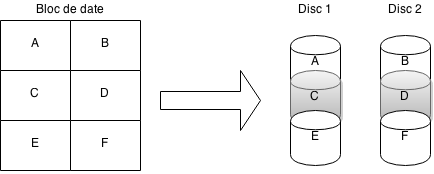
\includegraphics[width=0.6\textwidth]{img/raid0.png}
	\caption{Procesul de striping aplicat unui bloc de date}
	\end{center}
	\bigskip
\end{figure}

PASIS folose\c{s}te schemele de partajare pentru a distribui informa\c{t}ia nodurilor de stocare dintr-o re\c{t}ea. Aceasta introduce agen\c{t}i pe partea clientului pentru a scrie sau \c{s}terge date din noduri, dar \c{s}i agen\c{t}i pentru mentenan\c{t}\u{a}. Componentele obt\c{i}nute \^{i}n urma partaj\u{a}rii unui fisier sunt stocate in re\c{t}ea cu ajutorul agen\c{t}ilor (Fig. \ref{fig:pasis}). Pe l\^{a}ng\u{a} con\c{t}inutul brut al componentelor se adaug\u{a} metadate pentru a re\c{t}ine adresa nodului din re\c{t}ea la care au fost stocate dar \c{s}i noua denumire cu care este salvat\u{a} in re\c{t}ea.

Consider\^{a}nd o schem\u{a} de partajare majoritar\u{a} $(k, n)$ unde oricare din cei $k$ participan\c{t}i pot reconstitui fisierul, dar mai pu\c{t}in de $k$ nu ob\c{t}in nicio informa\c{t}ie dintr-un total de $n$ componente. 

Atunci c\^{a}nd un participant ini\c{t}iaz\u{a} o cerere pentru a citi un fisier, agentul PASIS aflat local procedeaz\u{a} dupa cum urmeaz\u{a}:
\begin{itemize}
	\item Caut\u{a} numele celor $n$ componente care alc\u{a}tuiesc fi\c{s}ierul \^{i}ntr-un serviciu care listeaz\u{a} toate datele.
	\item Ini\c{t}iaza cereri de citire la cel pu\c{t}in $k$ din cele $n$ noduri.
	\item \^{I}n caz ca acesta nu prime\c{s}te cel pu\c{t}in $k$ r\u{a}spunsuri se \^{i}ntoarce la pasul anterior \^{i}ncerc\^{a}nd interog\u{a}ri la noduri diferite.
	\item Reconstituie fi\c{s}ierul ob\c{t}inut din cele $k$ componente.
\end{itemize}
Opera\c{t}ia de scriere este similar\u{a} cu cea de citire, aceasta oprindu-se atunci c\^{a}nd \^{i}n cel pu\c{t}in $n - k + 1$ noduri s-au stocat cu succes componente.
\^{I}n articol se men\c{t}ioneaz\u{a} \c{s}i compromisul de spa\c{t}iu-timp folosit de PASIS \^{i}n func\c{t}ie de alegerea schemei de partajare. Spre exemplu, cererile de citire pot fi f\u{a}cute la acele $k$ noduri pentru care r\u{a}spunsurile recente au fost cele mai rapide.
Autorii specific\u{a} solu\c{t}ii pentru auto mentenan\c{t}a sistemului cu ajutorul resurselor umane prin monitorizarea periodic\u{a} st\u{a}rii sistemului folosind log-uri sau ajustarea parametrilor din cadrul schemei de partajare.

\begin{figure}
	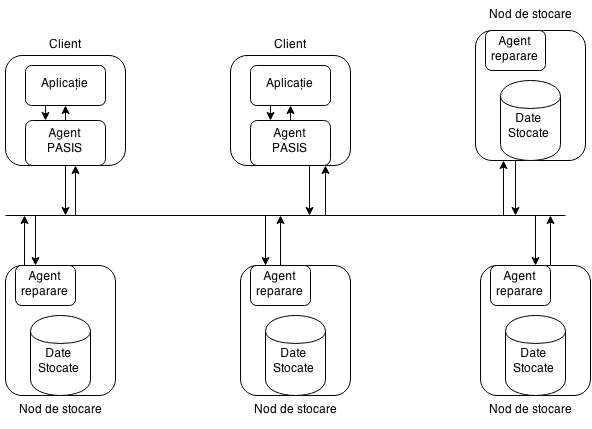
\includegraphics[width=11cm]{img/PASIS.png}
	\caption{Arhitectura PASIS cu $4$ noduri \c{s}i $2$ clien\c{t}i \cite{W:2000}.}
	\label{fig:pasis}
	\bigskip
\end{figure}

\subsection{GridSharing} 
\label{sec:desc_gridsharing}

\^{I}n 2005, Subbiah \c{s}i Blough propun o nou\u{a} abordare pentru a construi un sistem de stocare securizat \c{s}i tolerant la erori numit GridSharing \cite{SB:2005}.

Schema Shamir nu ofer\u{a} siguran\c{t}\u{a} \^{i}n ceea ce prive\c{s}te detectarea sau actualizarea unor componente incorecte introduse de un atacator. Metoda cea mai des folosit\u{a} este determinarea validit\u{a}\c{t}ii componentelor prin utilizarea semn\u{a}turilor electronice. Aceasta este realizat\u{a} prin scheme de verificare non-interactive precum cea a lui Feldman construit\u{a} pe baza schemei Shamir \cite{Feldman:1987} (Fig. \ref{fig:feldman_scheme})

%---------------- Figure - feldman_scheme - START ------------------------
\begin{figure*}[h!]

\begin{tabular}{|p{\textwidth}|}
\hline

\\
\hspace{.1in}
\textbf{Ini\c{t}ializare}: 
	Folosind nota\c{t}iile din Fig. \ref{fig:shamir_scheme}, consider\u{a}m polinomul $f$ generat \^{i}n urma Schemei Shamir.
	\begin{itemize}
		\item Se alege un $g \in Z_q$ generator al lui $Z_q$;
	\end{itemize}
\medskip

\hspace{.1in}
\textbf{Generare}: Dealerul $\mathcal{D}$:
	\begin{itemize}
		\item Calculeaz\u{a} \textit{angajamentele}: $c_0 = g^S$, $c_j = g^{a_j}$, $j \in \{1,\dots,k\}$;
	\end{itemize}
\medskip

\hspace{.1in}
\textbf{Distribu\c{t}ie}: Dealerul $\mathcal{D}$:
	\begin{itemize}
		\item Distribuie \textit{angajamentele} $c_j$, $j \in \{0,\dots,k\}$ fiec\u{a}rui participant $i\in \{1,\dots,n\}$;
	\end{itemize}

\hspace{.1in}
\\
\hline
\end{tabular}

\caption{Schema Feldman \cite{Feldman:1987}}
\label{fig:feldman_scheme}
\end{figure*}
%---------------- Figure - feldman_scheme- STOP ------------------------

Pentru verificarea componentei $s_i = f(i)$, participantul $i$ probeaz\u{a} ecua\c{t}ia:

\begin{equation}
	g^{s_i} = c_0c_1^ic_2^{i^2} \dots c_t^{i^t} = \prod_{j=0}^k c_j^{i^j} = \prod_{j=0}^k g^{a_ji^j} = g^{\sum\limits_{j=0}^k a_ji^j} = g^{f(i)}
\end{equation}

Subbiah \c{s}i Blough folosesc un sistem care \^{i}nlocuie\c{s}te schemele de verificare cu o schem\u{a} de partajare unanim\u{a} XOR (consider\u{a}m cazul $q = 2$ \^{i}n Fig. \ref{fig:all_or_nothing}) pentru a p\u{a}stra securitatea construc\c{t}iei.
\^{I}n cazul detect\u{a}rii componentelor incorecte, este adoptat\u{a} o strategie de tipul replicate-and-voting.
Componentele sunt replicate pe un num\u{a}r mare de servere astfel \^{i}nc\^{a}t determinarea validit\u{a}\c{t}ii va fi stabilit\u{a} \^{i}n func\c{t}ie de num\u{a}rul de servere care le con\c{t}in.

Se identific\u{a} 3 tipuri de defec\c{t}iuni care pot ap\u{a}rea pe serverele unde sunt stocate datele:
\begin{itemize}
	\item Abandon\u{a}ri: un server este \textit{abandonat} dac\u{a} nu mai raspunde vreunui mesaj din re\c{t}ea \c{s}i s-a oprit din a mai efectua vreo opera\c{t}ie.
	\item Bizantine: atunci c\^{a}nd serverul nu respect\u{a} \^{i}ntotdeauna protocoalele ini\c{t}iale iar componentele salvate local au fost compromise.
	\item Scurgeri de informa\c{t}ii: serverul execut\u{a} protocoalele corect dar e posibil ca un adversar s\u{a} fi ob\c{t}inut componentele stocate.
\end{itemize}
Primele 2 modele definite mai sus sunt preluate din calculul cu sisteme distribuite. Cel de-al 3-lea model a fost introdus pentru a defini atacatorul care folose\c{s}te vulnerabilit\u{a}\c{t}ile cu inten\c{t}ia de a \textit{\^{i}nva\c{t}a} din informa\c{t}ii.

Arhitectura GridSharing const\u{a} in $N$ servere unde cel mult $c$ servere pot fi abandonate, $b$ servere bizantine \c{s}i $l$ cu scurgeri de informa\c{t}ii. Cele $N$ pot fi aranjate \^{i}ntr-un grid cu $r$ linii \c{s}i $N/r$ coloane (consider\u{a}m pentru simplitate c\u{a} $N \Mod r = 0$). Caracteristicile modelului bizantin \c{s}i cel specific scurgerilor de informa\c{t}ii permit dezv\u{a}luirea componentelor unui adversar de pe cel mult $l + b$ servere.

\begin{example}

	Not\u{a}m ${x \choose y}$ fiind combin\u{a}ri de $x$ elemente grupate c\^{a}te $y$.
	Consider\u{a}m ca \^{i}mpar\c{t}im un secret $\mathcal{S}$ la $4$ linii (participan\c{t}i) astfel \^{i}nc\^{a}t sistemul s\u{a} permit\u{a} $2$ componente de tip $b$, $1$ component\u{a} de tip $l$ \c{s}i $20$ servere. \^{I}n cazul acesta vom folosi o schem\u{a} majoritar\u{a} XOR $\big( {4 \choose 3}, {4 \choose 3}\big) = (4,4)$.

	Vom avea $4$ componente, $(s_1, s_2, s_3, s_4)$ a.\^{i}. $s_1 \oplus s_2 \oplus s_3 \oplus s_4 = \mathcal{S}$.
	Distribuirea se face in felul urm\u{a}tor:
	\begin{itemize}
		% avem asa: p1, p2, p3, p4; s1, s2, s3
		% (p1 p2 p3, p1 p2 p4, p1 p3 p4, p2 p3 p4)
		% p1 | s4
		% p2 | s3
		% p3 | s2
		% p4 | s1
		\item Serverele situate pe prima linie primesc $s_1$
		\item Serverele situate pe a $2$-a linie primesc $s_2$
		\item Serverele situate pe a $3$-a linie primesc $s_3$
		\item Serverele situate pe a $4$-a linie primesc $s_4$
	\end{itemize}
\end{example}

\begin{figure}[H]
	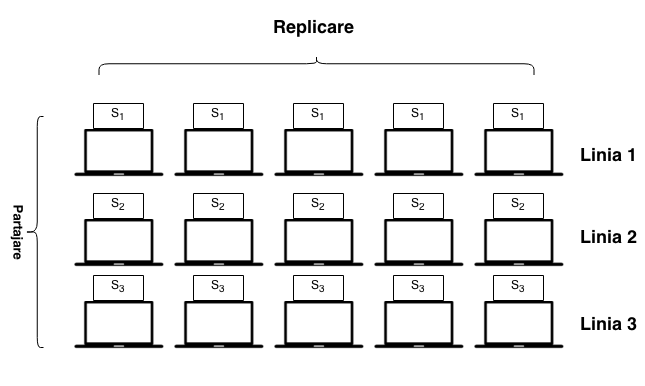
\includegraphics[width=12cm]{img/GridSharing.png}    % The printed column width is 8.4 cm.
	\caption{GridSharing cu $4$ linii, $20$ servere dintre care $2$ bizantine, $1$ cu scurgeri de informa\c{t}ii \cite{SB:2005}.}
	\label{fig:grid_sharing}
	\bigskip
\end{figure}


\subsection{POTSHARDS} 
\label{sec:desc_potshards}
\^{I}n $2007$ este propus un nou sistem care combin\u{a} caracteristicile PASIS \c{s}i GridSharing ad\u{a}ug\^{a}nd posiblitatea de migrarea a datelor la noduri noi: POTSHARDS (Protection Over Time, Securely Harboring And Reliably Distributing Stuff) \cite{SGMV:2009}.


POTSHARDS poate fi g\^{a}ndit ca o aplica\c{t}ie pe partea clientului care comunic\u{a} cu o mul\c{t}ime de noduri (arhive) independente, folosind reconstruc\c{t}ia componentelor \^{i}ntr-un mod securizat \c{s}i semn\u{a}turi algebrice pentru a asigura un grad ridicat de p\u{a}strare a integrita\c{t}ii fi\c{s}ierelor \cite{STM:2006}.

Confiden\c{t}ialitatea este asigurat\u{a} prin adoptarea unei scheme de partajare XOR unanim\u{a}, la fel ca \^{i}n GridSharing.

Ca prim pas, POTSHARDS preproceseaz\u{a} fi\c{s}ierul \^{i}ntr-un obiect, partajeaz\u{a} obiectul \^{i}n fragmente la care adaug\u{a} meta-date, numite \textit{shards} (Fig. \ref{fig:data-potshard}) \cite{SGMV:2009}. Acestea sunt trimise apoi arhivelor independente, fiecare av\^{a}nd propriul domeniu de securitate, localizate in \textit{regiuni}. Pentru a reconstitui cu succes informa\c{t}ia ini\c{t}ial\u{a}, meta-datele shard-urilor con\c{t}in detalii despre structura pointerilor aproximativi, indic\^{a}nd regiunea \^{i}n care se afl\u{a} urm\u{a}torul shard. Pointerii aproximativi sunt folositi pentru a reconstitui intreaga arhiva doar din shard-uri.

\begin{figure}
	\begin{center}
	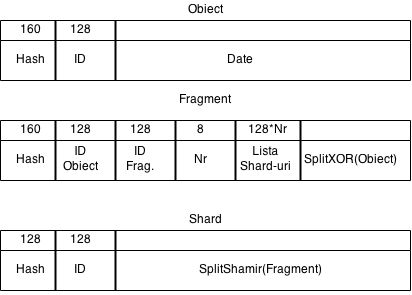
\includegraphics[width=7cm, height=4cm]{img/Shards.png}    % The printed column width is 8.4 cm.
	\caption{Entit\u{a}\c{t}i de date in POTSHARDS. $Nr$ e num\u{a}rul de shard-uri produse de un fragment.
		$SplitXOR$ reprezint\u{a} o component\u{a} rezultat\u{a} \^{i}n urma partajarii unanime XOR. Analog $SplitShamir$ reprezint\u{a} o component\u{a} rezultat\u{a} \^{i}n urma part\u{a}jarii folosind schema Shamir. \cite{SGMV:2009}}
	\label{fig:data-potshard}
	\bigskip
	\end{center}
\end{figure}

Procesul de fragmentare a datelor este prezentat in Fig. \ref{fig:potshards-layers}.

\begin{figure}
	\begin{center}
	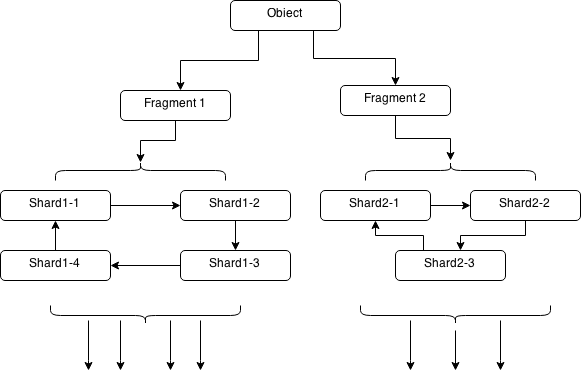
\includegraphics[width=12cm]{img/POTSHARDS.png}    % The printed column width is 8.4 cm.
	\caption{Distribuirea unui obiect in POTSHARDS}
	\label{fig:potshards-layers}
	\bigskip
	\end{center}
\end{figure}

Pentru ca reconstituirea unui fi\c{s}ier sa fie fezabil\u{a} unui utilizator, acestuia \^{i}i este \^{i}ntoars\u{a} o list\u{a} cu loca\c{t}iile exacte shard-urilor corespunz\u{a}toare.
Ob\c{t}inerea unui shard de c\u{a}tre un atacator nu este folositoare, pentru a detecta urm\u{a}torul shard, un atac brut force const\u{a} \^{i}n cereri multiple \^{i}n zona indicat\u{a} de pointerul aproximativ. Un astfel de atac nu va trece neobservat de POTSHARDS deorece unul dintre scopurile sale este s\u{a} stocheze datele \^{i}ntr-un mod cat mai uniform distribuit.\cite{SGMV:2009}

\section{Sistemul de stocare Alouneh et al.}
\label{sec:desc_alouneh}

Alouneh et al. propun un sistem pentru stocarea sigur\u{a} a datelor un timp indelungat folosind schema Shamir cu c\^{a}teva modific\u{a}ri. Aceste schimb\u{a}ri se vor ar\u{a}ta esen\c{t}iale mai t\^{a}rziu \^{i}n men\c{t}inerea securit\u{a}\c{t}ii \cite{AAMK:2013}.

Pentru stocarea unui fi\c{s}ier \^{i}n sistem (abord\^{a}nd filozofia majorit\u{a}\c{t}ii sistemelor de operare - orice este un fi\c{s}ier), o aplica\c{t}ie client \^{i}l \^{i}mparte \^{i}n blocuri de octe\c{t}i de lungime $k$. Pentru fiecare bloc, octe\c{t}ii devin coeficien\c{t}ii unui polinom $f$ de grad $k$, componenta corespunz\u{a}toare participantului $i$ va fi reprezentat\u{a} de valoarea lui $f(i)$, $i = \{1,2,\dots, n\}$. 
Men\c{t}ion\u{a}m c\u{a} toate opera\c{t}iile se vor efectua in $GF(256)$ modulo un polinom ireductibil (\^{i}n implementarea sistemului, autorii folosesc $x^8 + x^5 + x^3 + x + 1$). Procedeul este descris in detaliu in Fig \ref{fig:alouneh_distribution}.


%---------------- Figure - alouneh-distribution - START ------------------------
\begin{figure*}[h!]

\begin{tabular}{|p{\textwidth}|}
\hline

\\
\hspace{.1in}
\textbf{Date de intrare}: Un fi\c{s}ier binar $\mathcal{S}$;
\medskip

\hspace{.1in}
\textbf{Date de ie\c{s}ire}: $n$ fi\c{s}iere binare distribuite la noduri din re\c{t}ea;
\medskip

\hspace{.1in}
\textbf{Procesarea componentelor}: Aplica\c{t}ia existent\u{a} pe partea clientului: 
	\begin{itemize}
		\item Dac\u{a} $\mathcal{S}$ nu are o lungime divizibil\u{a} cu $k$:
			\begin{itemize}
			\item Concateneaz\u{a} la sf\^{a}rsitul lui $\mathcal{S}$ octe\c{t}i p\^{a}n\u{a} c\^{a}nd $len(\mathcal{S}) \Mod k = 0$;
			\end{itemize}
		\item \^{I}mparte $\mathcal{S}$ \^{i}n blocuri de lungime $k$;
		\item Repet\u{a} pentru fiecare bloc $B_t$ de lungime $k$:
		\begin{itemize}
			\item Construie\c{s}te polinomul $f(x) = B_{t_{k - 1}}x ^ {k-1} + B_{t_{k - 2}}x ^ {k - 2} + .... + B_{t_1}x + B_{t_0}$;
			\item Calculeaz\u{a} $f(i)$ pentru $1 \leq i \leq n$;
		\end{itemize}
	\end{itemize}

\hspace{.1in}
\textbf{Distribu\c{t}ie}: Aplica\c{t}ia la nivelul clientului:
	\begin{itemize}
		\item Distribuie componenta $f(i)$ nodului din re\c{t}ea cu indicele $i$:
	\end{itemize}

\\
\hline
\end{tabular}
\caption{Schema Alouneh et al. - Generare \cite{AAMK:2013}}
\label{fig:alouneh_distribution}
\end{figure*}

%---------------- Figure - alouneh_distribution - STOP ------------------------

\begin{example}
Vom exemplifica modul de calcul \^{i}n $GF(256) \Mod {g(x)} $ unde $g(x) = x ^ 8 + x ^ 4 + x ^ 3 + 1$. Lu\u{a}m polinomul $f(x) = 10 + 15x$ corespunz\^{a}tor unui fi\c{s}ier format din octe\c{t}ii (\^{i}n aceast\u{a} ordine) $10$ $15$.
	\begin{equation} \label{eq:f_01}
	\begin{split}
		f(01) \Mod{g(x)} & = 10 + 15 \Mod{g(x)} \\
		& = (x ^ 4) + (x ^ 4 + x ^ 2 + 1) \Mod{g(x)} \\
		& = x ^ 2 + 1 = 000000101_{(2)} \\
		& =  05_{(16)}
	\end{split}
	\end{equation}

	\begin{equation} \label{eq:f_02}
	\begin{split}
	 f(02) \Mod{g(x)} & = 10 + 15\cdot02 \Mod{g(x)} \\
	 & = (x ^ 4) + (x ^ 5 + x ^ 3 + x) \Mod{g(x)} \\
	 & = 00111010_{(2)} \\
	 & = 3A_{(16)}
	 \end{split}
	 \end{equation}
\end{example}
Reconstituirea unui fi\c{s}ier (Fig. \ref{fig:alouneh_reconstruction}) se realizeaz\u{a} din orice mul\c{t}ime de componente $A$ de dimensiune minim $k$ folosind interpolarea Lagrange (utilizat\u{a} \c{s}i \^{i}n cadrul schemei Shamir):
\begin{equation}
	\label{eq:lagrange_poly}
	f(x)=\sum_{i \in A} f(i) \prod_{j \in A, j \neq i} \frac{x-j}{i-j}
\end{equation}

\begin{example}
Vom exemplifica interpolarea conform ecua\c{t}iei {\ref{eq:lagrange_poly}} folosind componentele (\ref{eq:f_01}) \c{s}i (\ref{eq:f_02}) calculate \^{i}n exemplul anterior:
	\begin{equation}
	\begin{split}
		f(x) & = 05(x - 02)(01 - 02)^{-1} + 3A(x - 01)(02 - 01)^{-1} \\
		& = 05(x - 02)03^{-1} + 3A(x - 01)03^{-1} \\
		& = F6(05 + 3A)x + F6(05\cdot02 + 3A \cdot 01) \\
		& = F6\cdot 3F\cdot x + F6\cdot30 = 15x + 10
	\end{split}
	\end{equation}
\end{example}

Noutatea arhitecturii const\u{a} in diminuarea redundan\c{t}ei componentelor la un factor de $k$, spre deosebire de sistemele descrise in Sec\c{t}iunile \ref{sec:desc_pasis}, \ref{sec:desc_gridsharing} \c{s}i \ref{sec:desc_potshards}. Reducerea spa\c{t}iului ocupat de componente este datorat \^{i}nlocuirii coeficien\c{t}ilor genera\c{t}i aleator din schema Shamir cu octe\c{t}ii din fi\c{s}ierul ce va fi partajat, fiecare component\u{a} av\^{a}nd nevoie de $1/k$ din dimensiunea fi\c{s}ierului $\mathcal{S}$.

Abordarea acestei metode deterministe conduce la insecuritatea sistemului, Alouneh et al. afirm\^{a}nd \^{i}n mod eronat c\u{a} securitatea este indus\u{a} \^{i}n mod automat de schema Shamir. 

%---------------- Figure - alouneh-reconstruction- START ------------------------
\begin{figure*}[h!]

\begin{tabular}{|p{\textwidth}|}
\hline

\\
\hspace{.1in}
\textbf{Date de intrare}: Cel pu\c{t}in $k$ componente provenite din noduri (distincte);
\medskip

\hspace{.1in}
\textbf{Date de ie\c{s}ire}: Fi\c{s}ierul binar original $\mathcal{S}$;
\medskip

\hspace{.1in}
\textbf{Reconstruc\c{t}ie}: Aplica\c{t}ia existenta pe partea clientului: 
	\begin{itemize}
		\item Repet\u{a} pentru fiecare bloc al lui $\mathcal{S}$:
		\begin{itemize}
			\item Calculeaz\u{a} prin interpolare coeficien\c{t}ii lui $f(x)=B_{t_{k - 1}}x ^ {k-1} + B_{t_{k - 2}}x ^ {k - 2} + .... + B_{t_1} + B_{t_0}$
			\item Reconstituie blocul $B_t$
		\end{itemize}
		\item \c{S}terge octe\c{t}ii de la sf\^{a}r\c{s}itul fi\c{s}ierului ad\u{a}uga\c{t}i la generare. 
	\end{itemize}

\\
\hline
\end{tabular}
\caption{Schema Alouneh et al. - Reconstruc\c{t}ie \cite{AAMK:2013}}
\label{fig:alouneh_reconstruction}
\end{figure*}

%---------------- Figure - alouneh_reconstruction- STOP ------------------------

%\todo{poti incerca sa adaugi si aici o imagine}


%----------------------------------------------------------------
%----------------------------------------------------------------
%----------------------------------------------------------------
%----------------------------------------------------------------
%----------------------------------------------------------------

\section{Rezultate ob\c{t}inute}
\label{sec:obtained_results}

\^{I}mpreun\u{a} cu mentorul am analizat sistemul Alouneh et al. prezentat \^{i}n Sec\c{t}iunea \ref{sec:desc_alouneh} \cite{AAMK:2013}.
 Am indentificat erori majore ale acestuia \c{s}i am implementat sistemul descris de autori pentru a demonstra practic, nu doar teoretic anumite gre\c{s}eli pe care le vom eviden\c{t}ia \^{i}n urm\u{a}toarele sec\c{t}iuni.

\subsection{Vulnerabilit\u{a}\c{t}i eviden\c{t}iate}

Spre deosebire de schema Shamir, unde coeficien\c{t}ii (cu excep\c{t}ia termenului liber, care este egal cu secretul) sunt ale\c{s}i \^{i}ntr-un mod aleator uniform, sistemul propus de Alouneh et al. folose\c{s}te o schem\u{a} modificat\u{a} Shamir \^{i}n care coeficien\c{t}ii sunt extra\c{s}i din con\c{t}inutul fi\c{s}ierelor originale.
Alegerea este motivat\u{a} de faptul ca mul\c{t}imea componentelor \c{s}i efortul computa\c{t}ional depus pentru generarea coeficien\c{t}ilor se reduce la un factor de $k$ ori, spre deosebire de schema Shamir.

Datorit\u{a} determinismului, partajarea unui fi\c{s}ier de mai multe ori implic\u{a} ob\c{t}inerea de componente identice.
Determinismul duce la c\^{a}teva atacuri simple \^{i}n momentul \^{i}n care un atacator ob\c{t}ine informa\c{t}iile stocate \^{i}ntr-un nod, indiferent de m\u{a}rimea pragului folosit \^{i}n metoda de partajare. \^{I}n acest sens, am eviden\c{t}iat $2$ atacuri simple \^{i}n cazul \^{i}n care componentele sunt calculate in ordine ($f(01), f(02), \dots$):
\begin{itemize}
	\item Detectarea tipului unui fi\c{s}ier
	\item Detectarea con\c{t}inutului unui fi\c{s}ier
\end{itemize}

Deoarece Alouneh et al. nu men\c{t}ionea\u{a} o metoda de padding, am indicat c\u{a} un atac bazat pe felul \^{i}n care se realizeaz\u{a} completarea fi\c{s}ierului (padding) $\mathcal{S}$ \^{i}nainte de partajarea sa poate fi fezabil, \^{i}n condi\c{t}iile \^{i}n care s-a demonstrat ca aceast\u{a} alegere este esen\c{t}ial\u{a} \^{i}n p\u{a}strarea securit\u{a}\c{t}ii \cite{Vaudenay:2002}.

\subsubsection{Detectarea tipului de fi\c{s}ier}\hspace*{\fill} \\
\label{subsec:file_type_detection}

\^{I}n tehnologia informa\c{t}iei, la inceputul fiec\u{a}rui fi\c{s}ier se afl\u{a} o secven\c{t}\u{a} de octe\c{t}i (denumit\u{a} semnatur\u{a} sau antet) cu rolul de a identifica tipul acestuia. Tabelul {\ref{table:sign}} indic\u{a} $7$ din cele mai uzuale antete.

Se consider\u{a} cazul \^{i}n care partajarea unui fi\c{s}ier \textit{pdf} se face cu ajutorul sistemului descris in {S}ec\c{t}iunea \ref{sec:desc_alouneh}, folosind $k \leq 4$. Polinomul corespunz\u{a}tor $f(x)$ va fi intotdeauna acela\c{s}i. Presupun\^{a}nd ca numerotarea nodului $i$ este aceea\c{s}i, putem determina cu u\c{s}urin\c{t}\u{a} dac\u{a} este stocat un fi\c{s}ier \textit{pdf} f\u{a}r\u{a} a lua \^{i}n calcul con\c{t}inutul fi\c{s}ierului.
Acest atac este fezabil deorece valoarea lui $k$ este public\u{a} iar $i$ poate sa fie descoperit \^{i}n momentul distribuirii.

Cu alte cuvinte, dac\u{a} un adversar obt\c{i}ne controlul unui singur nod, baz\^{a}ndu-se doar pe valoarea primei componente poate detecta tipul unui fi\c{s}ier.

Pentru a exemplifica, un adversar poate distinge cu probabilitate ridicat\u{a} \^{i}ntre fi\c{s}ierele \textit{doc, gif, pdf, png, rar, wav} \c{s}i \textit{zip}. \^{I}n Tabelul {\ref{table:shares}} avem generate componentele pentru $k = 2$ \c{s}i $n = 5$.
Dac\u{a} un adversar descoper\u{a} valoarea primului nod iar prima component\u{a} este $14$ atunci acesta \c{s}tie cu certitunde c\u{a} aceasta corespunde un fi\c{s}ier \textit{gif}. Dac\u{a} ob\c{t}ine accesul nodului $4$ \c{s}i cite\c{s}te valoarea $205$ atunci \c{s}tie c\u{a} fi\c{s}ierul este de tipul \textit{rar}. Daca cite\c{s}te valoarea $27$ de pe primul nod atunci \c{s}tie c\u{a} poate fi un \textit{wav} sau \textit{zip}; dar poate s\u{a} disting\u{a} cele 2 fi\c{s}iere cu probabilitate $1$ dac\u{a} dezv\u{a}luie o singur\u{a} valoare de pe celelalte noduri ($2$, $3$, $4$ sau $5$) pentru c\u{a} valorile sunt distincte.

%-----------------------------------------------------
\begin{table}
\bigskip
\begin{center}
\caption{Semn\u{a}turi de fi\c{s}iere}\label{tb:margins}
\label{table:sign}
\begin{tabular}{ccccc}
Tip de fi\c{s}ier &  \multicolumn{4}{c}{Primii 4 octe\c{t}i}\\ \hline 
doc &  D0 & CF & 11 & E0\\
gif & 47 & 49 & 46 & 38 \\
pdf & 25 & 50 & 44 & 46 \\
png & 89 & 50 & 4E & 47 \\
rar & 52 & 61 & 72 & 21 \\
wav & 52 & 49 & 46 & 46 \\
zip & 50 & 4B & 03 & 04\\  \hline
\end{tabular}
\end{center}
\bigskip
\end{table}

%-----------------------------------------------------
\begin{table}
\begin{center}
\caption{Componentele primului bloc ($k=2$)}\label{tb:margins}
\label{table:shares}
\begin{tabular}{cccccccc}
Tip fisier & Nod 1 & Nod 2 & Nod 3 & Nod 4 & Nod 5 \\
  & ($i=1$) & ($i=2$) & ($i=3$) & ($i=4$) & ($i=5$) \\
\hline
doc & 31 & 85 & 154 & 193 & 14 \\
gif & 14 & 213 & 156 & 120 & 49 \\
pdf & 117 & 133 & 213 & 126 & 46 \\
png & 217 & 41 & 121 & 210 & 130 \\ 
rar & 51 & 144 & 241 & 205 & 172  \\
wav & 27 & 192 & 137 & 109 & 36 \\
zip & 27 & 198 & 141 & 103 & 44 \\ \hline
\end{tabular}
\end{center}
\bigskip
\end{table}

%-----------------------------------------------------

\subsubsection{Detectarea de con\c{t}inut}\hspace*{\fill} \\
\label{subsec:file_content_detection}

Multe documente urmeaz\u{a} un anumit tipar precum contracte, chitan\c{t}e, bonuri fiscale sau curriculum vitae. Deoarece majoritatea con\c{t}inutului r\u{a}m\^{a}ne neschimbat, exist\u{a} o probabilitate destul de mare ca multe componente sa aiba aceea\c{s}i valoare. O dat\u{a} ce un adversar reu\c{s}e\c{s}te s\u{a} determine componentele unui nod, poate determina prin analogie tipul de con\c{t}inut al fi\c{s}ierului original.

Fi\c{s}ierele vulnerabile sunt cele care con\c{t}in o secven\c{t}\u{a} de octe\c{t}i periodic\u{a} (imagini cu un pattern repetitiv) sau cele care au preponderent octe\c{t}i nuli (valoarea componentelor asociat\u{a} majorit\u{a}\c{t}ii blocurilor fiind $0$). Spre deosebire de prima metod\u{a}, aceasta nu necesit\u{a} compararea cu un al $2$-lea fi\c{s}ier, trat\^{a}nd componentele de sine st\u{a}t\u{a}tor. Multiple componente identice indic\u{a} existen\c{t}a unor secven\c{t}e repetitive \^{i}n con\c{t}inutul fi\c{s}ierului.

\subsection{Implementare \c{s}i rezultate practice}
Pentru a ar\u{a}ta aplicabilitatea rezultatelor \^{i}n practic\u{a}, am implementat propunerea descrisa in Sec\c{t}iunea {\ref{sec:desc_alouneh}} \c{s}i am testat pe c\^{a}teva cazuri.

\^{I}n cadrul implement\u{a}rii am folosit limbajul Python 3.0 sub sistemul de operare ArchLinux. Python este un limbaj high-level, permi\c{t}\^{a}nd programatorilor s\u{a} exprime concepte \^{i}n mai pu\c{t}ine linii de cod fa\c{t}\u{a} de C++ sau Java \c{s}i este disponibil sub licen\c{t}\u{a} open-source \cite{Python:2015}.
Pentru a realiza comunicarea \^{i}ntre procese am folosit Cerealizer iar distribu\c{t}ia componentelor a fost generat\u{a} grafic cu ajutorul pachetului Matplotlib \cite{Hunter:2007, PyCerealizer:2015}. De asemenea am folosit sistemul de versionare Git iar \^{i}n prezent codul folosit este g\u{a}zduit de GitHub \cite{Github:2015, CodeGit:2015}.

Av\^{a}nd \^{i}n vedere c\u{a} articolul original nu men\c{t}ioneaz\u{a} o metod\u{a} de padding, am considerat o metod\u{a} standard pentru a completa octe\c{t}ii ultimului bloc: alipim la sf\^{a}r\c{s}itul lui $\mathcal{S}$ octe\c{t}ii $80$ $00$ $\dots$ $00$ $00$ p\^{a}n\u{a} c\^{a}nd lungimea ultimului bloc ajunge la $k$ octe\c{t}i.

Men\c{t}ion\u{a}m aceast\u{a} metoda doar pentru completitudine, aceasta neafect\^{a}nd rezultatele, care consider\u{a} doar secven\c{t}ele de octe\c{t}i din antet sau de la \^{i}nceputul fi\c{s}ierului.

\subsubsection{Detectarea tipului de fi\c{s}ier}\hspace*{\fill} \\

Extindem analiza f\u{a}cut\u{a} \^{i}n Sec\c{t}iunea {\ref{subsec:file_type_detection}} asupra tipurilor de fi\c{s}iere din Tabelul {\ref{table:sign}} pentru $k = 2$ \c{s}i cre\c{s}tem valoarea indicelui $i$ p\^{a}n\u{a} c\^{a}nd 2 componente devin egale. Fie $f_l$ polinomul de gradul $1$ asociat primului bloc al fi\c{s}ierului aflat pe linia $l$. Analog $f_c$ polinomul de gradul $1$ asociat primului bloc al fi\c{s}ierului aflat pe coloana $c$.

Tabelul {\ref{table:k2} prezint\u{a}} valoarea maxim\u{a} a nodul $i$ pentru care $f_l(i) \neq f_c(i)$. Valoarea $-1$ indic\u{a} lips\u{a} de coliziuni ale lui $f_c(x)$, $f_l(x)$ pentru $i$, $i = {1,2,\dots,255}$ ($\not\exists 1 \leq i \leq 255$ a.\^{i}. $f_l(i) = f_c(i)$)).

Deoarece pe diagonala principal\u{a} toate componentele sunt identice pentru $k \leq 4$, poate fi ignorat\u{a}. \^{I}n Tabelul {\ref{table:k2}} observ\u{a}m valoarea $0$ pentru perechea $(wav, zip)$ pentru c\u{a} $f_{wav}(1) = f_{zip}(1) = 27$ (Tabelul \ref{table:sign}).

Tabelele {\ref{table:k3} \c{s}i \ref{table:k4}} prezint\u{a} rezultatele pentru $k = 3$ si $k = 4$. Pentru $k \geq 5$ este nevoie de un antet cu mai mult de $4$ octe\c{t}i.

Consider\u{a}m metoda de distribuire descris\u{a} exact ca \^{i}n Tabelul {\ref{fig:alouneh_distribution}}, \c{s}i anume nodul de stocare $i$ prime\c{s}te componenta $f(i)$.
Dac\u{a} un atacator preia controlul nodului cu valoarea $i$ acesta poate face distinc\c{t}ia \^{i}ntre tipul a $2$ fi\c{s}iere partajate cu probabilitate $1$ dac\u{a} $i$ e mai mic dec\^{a}t valoarea afi\c{s}at\u{a} \^{i}n tabel.

Spre exemplu, un adversar care ob\c{t}ine accesul unui singur nod de stocare, iar partajarea a fost f\u{a}cut\u{a} pentru $k=2$ poate distinge cu probabilitate $1$ \^{i}ntre un fi\c{s}ier $doc$ sau $pdf$ dac\u{a} $i \leq 194$. Deoarece $n > 194$ nu se \^{i}nt\^{a}mpl\u{a} \^{i}n practic\u{a}, acest atac func\c{t}ioneaz\u{a}. Faptul c\u{a} multe valori sunt ridicate \c{s}i majoritatea sunt $-1$ (Tabelul \ref{table:k3}), indic\u{a} un nivel sc\u{a}zut de securitate al schemei. \^{I}n cazul celor cu $-1$ un adversar va ca\c{s}tiga \^{i}ntotdeauna cu probabilitatea $1$, indiferent de indicele nodului de stocare pe care il ob\c{t}ine.

Preciz\u{a}m c\u{a} acest atac func\c{t}ioneaz\u{a} doar dac\u{a} nodurile de stocare \^{i}\c{s}i p\u{a}streaz\u{a} indexul \^{i}n cazul partaj\u{a}rii repetate a.\^{i}. aplica\c{t}ia disponibil\u{a} pe partea de client calculeaz\u{a} cele $n$ valori $f(i_1),\dots,f(i_2)$ pentru $i_1,\dots,i_n$ distincte \c{s}i p\u{a}streaz\u{a} nodul $j$ asociat lui $i_j$.


%-----------------------------------------------------
\begin{table}[b]
\begin{center}
\caption{Indicele maxim $i$ a.\^{i}. componentele primului bloc sa fie distincte($k=2$)}\label{tb:margins}
\label{table:k2}
\begin{tabular}{cccccccc}
Tip Fi\c{s}ier & doc & gif & pdf & png & rar & wav & zip \\\hline
  doc & - & 169 & 194 & 209 & 170 & 206 & 110\\
  gif & 169 & - & 133 & 137 & 75 & -1 & 133\\
  pdf & 194 & 133 & - & -1 & 115 & 151 & 133\\
  png & 209 & 137 & -1 & - & 229 & 147 & 195\\
  rar & 170 & 75 & 115 & 229 & - & -1 & 42\\
  wav & 206 & -1 & 151 & 147 & -1 & - & 0\\
  zip & 110 & 133 & 133 & 195 & 42 & 0 & -\\ \hline
\end{tabular}
\end{center}
\end{table}

%-----------------------------------------------------

\begin{table}[H]
\begin{center}
\caption{Indicele maxim $i$ a.\^{i}. componentele primului bloc sa fie distincte($k=3$)}\label{tb:margins}
\label{table:k3}
\begin{tabular}{cccccccc}
Tip Fi\c{s}ier & doc & gif & pdf & png & rar & wav & zip \\\hline
  doc & - & 63 & -1 & -1 & -1 & -1 & -1\\
  gif & 63 & - & -1 & -1 & -1 & -1 & -1\\
  pdf & -1 & -1 & - & 164 & -1 & 119 & -1\\
  png & -1 & -1 & 164 & - & 143 & 122 & 129\\
  rar & -1 & -1 & -1 & 143 & - & 143 & -1\\
  wav & -1 & -1 & 119 & 122 & 143 & - & 172\\
  zip & -1 & -1 & -1 & 129 & -1 & 172 & -\\ \hline
\end{tabular}
\end{center}
\bigskip
\end{table}

%-----------------------------------------------------
\begin{table}[H]
\begin{center}
\caption{Indicele maxim $i$ a.\^{i}. componentele primului bloc sa fie distincte($k=4$)}\label{tb:margins}
\label{table:k4}
\begin{tabular}{cccccccc}
Tip Fi\c{s}ier & doc & gif & pdf & png & rar & wav & zip \\\hline
  doc & - & -1 & 38 & 95 & 1 & 95 & 98\\
  gif & -1 & - & -1 & -1 & 167 & -1 & -1\\
  pdf & 38 & -1 & - & 12 & 11 & 119 & 70\\
  png & 95 & -1 & 12 & - & 243 & 95 & 148\\
  rar & 1 & 167 & 11 & 243 & - & -1 & 94\\
  wav & 95 & -1 & 119 & 95 & -1 & - & -1\\
  zip & 98 & -1 & 70 & 148 & 94 & -1 & -\\ \hline
\end{tabular}
\end{center}
\bigskip
\end{table}

\subsubsection{Detectarea de con\c{t}inut} \hspace*{\fill} \\

Consider\u{a}m scenariul pentru detectarea con\c{t}inutului unui fi\c{s}ier, demonstr\^{a}nd practic cum un adversar poate s\u{a} fac\u{a} diferen\c{t}a \^{i}ntre $2$ componente stocate pe acela\c{s}i nod apar\c{t}in unor documente similare. Atacul presupune accesul la un singur nod, indiferent de m\u{a}rimea pragului $k$.

Pentru experiment am ales $3$ fi\c{s}iere \textit{pdf} disponibile online la {\cite{Europass:2015}}:
\begin{itemize}
  \item Europass Curriculum Vitae - BG, Bulgaria;
  \item Europass Curriculum Vitae - DK, Dannemark;
  \item Europass Mobility - RO, Romania.
\end{itemize}

Primele dou\u{a} fi\c{s}iere reprezint\u{a} \c{s}ablonul pentru un CV european \^{i}n limba bulgar\u{a}, respectiv danez\u{a}. Observ\u{a}m c\u{a} nu doar con\c{t}inutul \c{s}abloanelor difer\u{a}, dar \c{s}i limba \^{i}n care au fost traduse. Cel de-al treilea fi\c{s}ier este complet diferit de primele dou\u{a}, fiind un document personal \^{i}n limba rom\^{a}n\u{a}, folosit pentru \^{i}nregistrarea cuno\c{s}tiintelor dob\u{a}ndite \^{i}ntr-o \c{t}ar\u{a} european\u{a}.

Pentru a ar\u{a}ta vulnerabilitatea sistemului Alouneh et al. {\cite{AAMK:2013}}, partaj\u{a}m cele $3$ fi\c{s}iere folosind schema $(2, 4)$. Experimentul reprezint\u{a} o implementare practic\u{a} a metodei prezentate in Fig. {\ref{fig:alouneh_distribution}}.


%-----------------------------------------------------

\begin{figure}[H]
\begin{center}{}
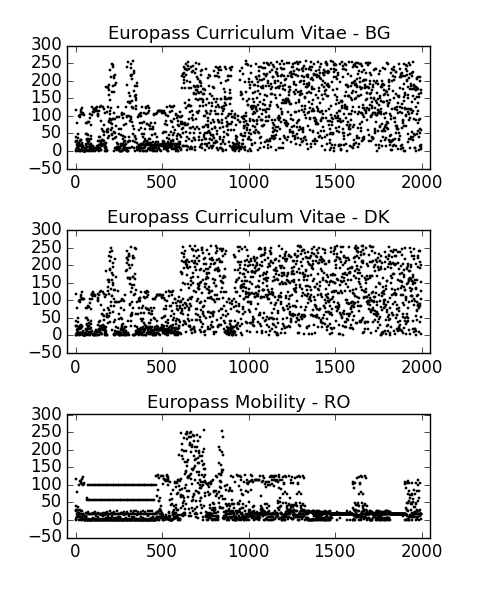
\includegraphics[width=0.6\textwidth]{img/db1.png}    % The printed column width is 8.4 cm.
\caption{Nod 1: Graficul componentelor pentru primele 2000 de blocuri} 
\label{fig:db1}
\end{center}
\end{figure}
%-----------------------------------------------------

%-----------------------------------------------------
\begin{figure}
\begin{center}
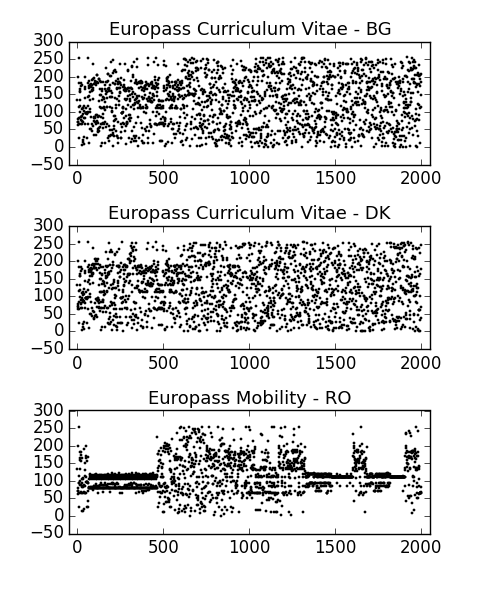
\includegraphics[width=0.6\textwidth]{img/db2.png}    % The printed column width is 8.4 cm.
\caption{Nod 2: Graficul componentelor pentru primele 2000 de blocuri} 
\label{fig:db2}
\end{center}
\end{figure}
%-----------------------------------------------------

%-----------------------------------------------------
\begin{figure}
\begin{center}
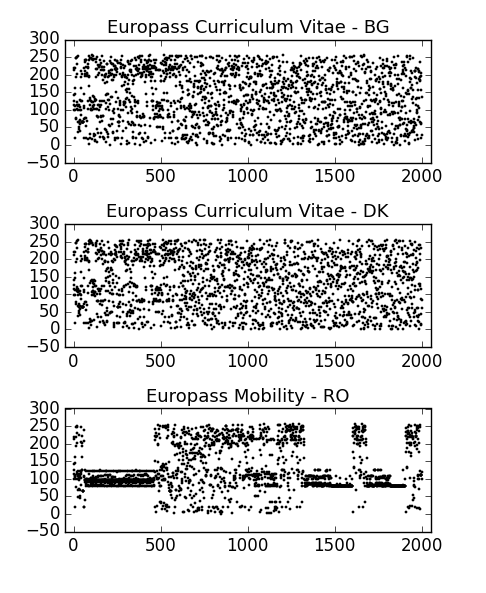
\includegraphics[width=0.6\textwidth]{img/db3.png}    % The printed column width is 8.4 cm.
\caption{Nod 3: Graficul componentelor pentru primele 2000 de blocuri} 
\label{fig:db3}
\end{center}
\end{figure}
%-----------------------------------------------------

%----------------------------------------------------
\begin{figure}
\begin{center}
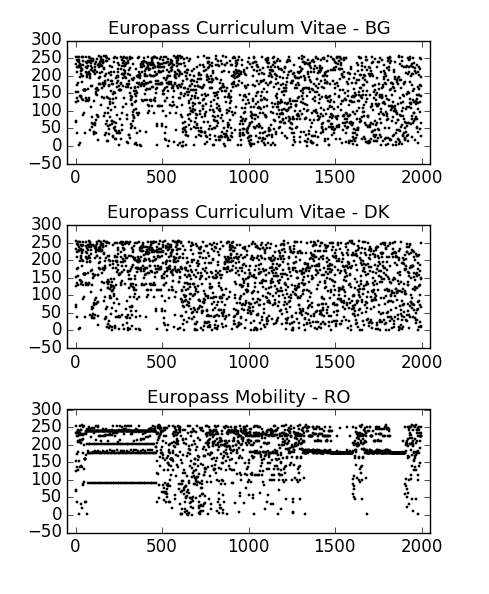
\includegraphics[width=0.6\textwidth]{img/db4.png}    % The printed column width is od8.4 cm.
\caption{Nod 4: Graficul componentelor pentru primele 2000 de blocuri} 
\label{fig:db4}
\end{center}
\end{figure}
%-----------------------------------------------------
%-----------------------------------------------------

Fig. {\ref{fig:db1}}, {\ref{fig:db2}}, {\ref{fig:db3}}, {\ref{fig:db4}} con\c{t}in $2000$ de componente generate pentru cele $3$ fi\c{s}iere, stocate \^{i}n baza de date corespunz\u{a}toare nodurilor $1,2,3$ \c{s}i $4$. Presupunem c\u{a} indicele $i$ este fixat, polinoamele fiind evaluate \^{i}n acela\c{s}i nod $i$. Un adversar care ob\c{t}ine componentele unui nod poate deduce cu u\c{s}urinta graficul lor.

Consider\u{a}m c\u{a} un adversar reu\c{s}e\c{s}te s\u{a} ob\c{t}in\u{a} componentele din Fig. {\ref{fig:db1}}. Poate deduce u\c{s}or c\u{a} primele dou\u{a} fi\c{s}iere au un num\u{a}r mare de componente identice iar cel de-al $3$-lea este diferit de primele.

Din cauza \c{s}ablonului pe care \^{i}l respect\u{a} cele dou\u{a} CV-uri, un adversar are nevoie \^{i}n cazul de fa\c{t}\u{a} doar de primele $500$ de componente pentru a constata similiaritatea celor $2$ cu o probabilitate ridicat\u{a}.
Diferen\c{t}a vizuala este evident\u{a} \^{i}ntre oricare din cele $4$ grafice, deci un adversar poate reu\c{s}i s\u{a} afle informa\c{t}ii despre fi\c{s}ierele partajate indiferent de nodul de stocare vulnerabil.

Consider\u{a}m \^{i}n continuare un alt scenariu, \^{i}n care partaj\u{a}m o imagine pentru care informa\c{t}ia se repet\u{a}. Fie imaginea din Fig. {\ref{fig:carouri}} partajat\u{a} folosind schema din Sec\c{t}iunea {\ref{sec:desc_alouneh}} av\^{a}nd $4$ noduri iar informa\c{t}ia stocat\u{a} pe cel pu\c{t}in $2$ din ele pot reconstitui imaginea partajat\u{a} ini\c{t}ial. {\ref{fig:alouneh_distribution}}. La fel ca \^{i}n exemplul precedent, Fig. {\ref{fig:carouri_db1}, \ref{fig:carouri_db2}, \ref{fig:carouri_db3}, \ref{fig:carouri_db4}} reprezint\u{a} grafic componente imaginii din Fig. {\ref{fig:carouri}}. Un adversar constat\u{a} cu u\c{s}urin\c{t}\u{a} prin ob\c{t}inerea informa\c{t}iilor stocate aflate pe un singur nod (indiferent de m\u{a}rimea pragului $k$) c\u{a} fi\c{s}ierul original con\c{t}ine un pattern care se repet\u{a}.


%-----------------------------------------------------
\begin{figure}[H]
\begin{center}

\includegraphics[width=0.35\textwidth]{img/carouri.png}    % The printed column width is 8.4 cm.
\caption{Imagine con\c{t}in\^{a}nd pattern-uri} 
\label{fig:carouri}
\end{center}
\end{figure}
%-----------------------------------------------------


%-----------------------------------------------------
\begin{figure}
\begin{center}
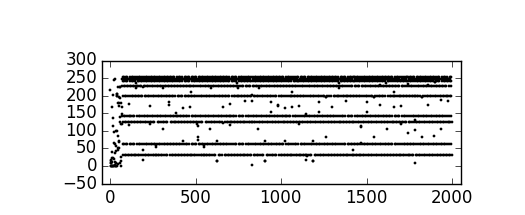
\includegraphics[width=0.5\textwidth]{img/carouri_db1.png}    % The printed column width is 8.4 cm.
\caption{Nod 1: Graficul componentelor pentru primele 2000 de blocuri} 
\label{fig:carouri_db1}
\end{center}
\end{figure}
%-----------------------------------------------------

%-----------------------------------------------------
\begin{figure}
\begin{center}
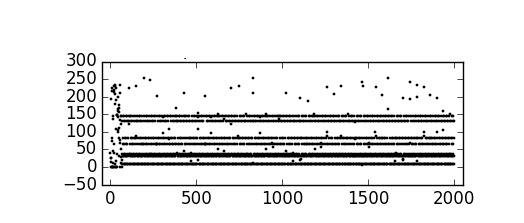
\includegraphics[width=0.5\textwidth]{img/carouri_db2.png}    % The printed column width is 8.4 cm.
\caption{Nod 2: Graficul componentelor pentru primele 2000 de blocuri} 
\label{fig:carouri_db2}
\end{center}
\end{figure}
%-----------------------------------------------------

%-----------------------------------------------------
\begin{figure}
\begin{center}
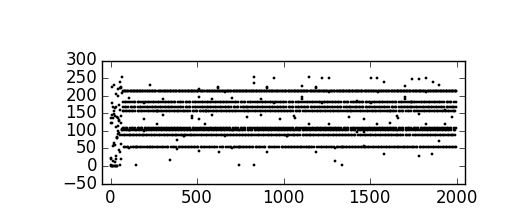
\includegraphics[width=0.5\textwidth]{img/carouri_db3.png}    % The printed column width is 8.4 cm.
\caption{Nod 3: Graficul componentelor pentru primele 2000 de blocuri} 
\label{fig:carouri_db3}
\end{center}
\end{figure}
%-----------------------------------------------------

%-----------------------------------------------------
\begin{figure}
\begin{center}
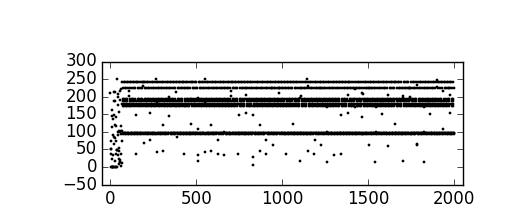
\includegraphics[width=0.5\textwidth]{img/carouri_db4.png}    % The printed column width is 8.4 cm.
\caption{Nod 4: Graficul componentelor pentru primele 2000 de blocuri} 
\label{fig:carouri_db4}
\end{center}
\end{figure}
%-----------------------------------------------------

\subsection{Publicarea rezultatelor}

Pe baza rezultatelor ob\c{t}inute am redactat (\^{i}mpreun\u{a} cu mentorul) un articol, aflat momentan \^{i}n procesul de recenzie la Journal of Control Engineering and Applied Informatics (jurnal indexat ISI,categoria C). \cite{Ceai:2015}
%
% ---- Bibliography ----
%
%\begin{thebibliography}{5}
%
\clearpage
\bibliographystyle{splncs}
\bibliography{llncs}
%\end{thebibliography}

\end{document}